\documentclass[11pt,a4paper]{article}

\usepackage[utf8]{inputenc}
\usepackage[T1]{fontenc}
\usepackage[portuguese]{babel}
\usepackage[margin=2.5cm]{geometry}
\usepackage{graphicx}
\usepackage{booktabs}
\usepackage{amsmath}
\usepackage{siunitx}
\usepackage[colorlinks=true, linkcolor=black, urlcolor=blue, citecolor=black]{hyperref}
\usepackage{float}

\sisetup{output-decimal-marker={,}}

\title{\textbf{Visualização e Iluminação --- Projeto 2025/26}\\[0.5em]
\large Temas: Motion Blur (6) \,\textperiodcentered\, Acceleration Structure: BVH (2) \,\textperiodcentered\, Depth of Field (5)}

\author{[NOME 1] ([número]) \and Gonçalo Barroso (PG58980) \and [NOME 3] ([número])\\[0.3em]
\small Mestrado em Engenharia Informática --- Universidade do Minho}

\date{\today}

\begin{document}

\maketitle

\section{Introdução}

O ponto de partida deste trabalho é o \emph{path tracer} desenvolvido nas aulas (VI-RT): um \emph{renderer} por traçado de raios com iluminação global, materiais difusos e metálicos, amostragem por importância da iluminação direta, carregamento de cenas glTF e \emph{denoising} final com Intel Open Image Denoise (OIDN)~\cite{oidn}.

Sobre esta base implementámos três temas complementares entre si:

\begin{itemize}
  \item \textbf{Motion Blur (tema 6)} --- desfoque de movimento: objetos em movimento durante o tempo de exposição aparecem com rasto, como numa fotografia real;
  \item \textbf{BVH (tema 2)} --- \emph{Bounding Volume Hierarchy}: estrutura de aceleração que reduz o custo de interseção raio--cena de $O(n)$ para $O(\log n)$;
  \item \textbf{Depth of Field (tema 5)} --- profundidade de campo: simulação de uma lente com abertura finita, mantendo nítido o plano focal e desfocando o resto.
\end{itemize}

Os três temas formam um todo coerente: o \emph{motion blur} e o \emph{depth of field} são efeitos \emph{estocásticos} --- exigem muitas amostras por pixel (spp) para convergir sem ruído --- e a BVH é a infraestrutura que torna esse custo praticável em cenas com muita geometria.

Salvo indicação em contrário, os resultados foram medidos a $1280\times720$, em \emph{single-thread}, \emph{build} Release. Cada tema pode ser executado diretamente na linha de comandos: \texttt{VI-RT motion-blur}, \texttt{VI-RT bvh}, \texttt{VI-RT sponza}, com as opções \texttt{--spp N} (amostras por pixel) e \texttt{--accel bvh|grid} (estrutura de aceleração).

% ============================================================================
% ========================== TEMA 6 — MOTION BLUR ============================
% ====================== [SECÇÃO DE: ] =========================
% ============================================================================

\section{Tema 6 --- Motion Blur}
\label{sec:motionblur}

% TODO [colega]: escreve aqui a tua parte. Estrutura sugerida (igual à do tema 2):

\subsection{Fundamento}

% TODO [colega]: o que é o motion blur e como se simula num path tracer
% (tempo aleatório por raio, referência: Ray Tracing The Next Week \cite{rtnw}).

[A preencher.]

\subsection{Implementação}

% TODO [colega]: campo Time no Ray, amostragem do tempo na Camera,
% Sphere com dois centros e interpolação, bounding box = união de t=0 e t=1,
% cena de demonstração (VI-RT motion-blur).

[A preencher.]

\subsection{Resultados}

% TODO [colega]: a figura está pronta em report-assets/motion-blur.png
% (64 spp + OIDN, render de 44,9 s). Descomenta o bloco abaixo e escreve a análise.

% \begin{figure}[H]
%   \centering
%   \includegraphics[width=0.78\textwidth]{motion-blur.png}
%   \caption{Cena de \emph{motion blur}, 64 spp + OIDN. As esferas pequenas em
%   movimento exibem rasto vertical; as esferas grandes, estáticas, permanecem nítidas.}
%   \label{fig:motionblur}
% \end{figure}

[A preencher.]

% ============================================================================
% ============================ TEMA 2 — BVH ==================================
% ======================= [SECÇÃO DE: Gonçalo Barroso] =======================
% ============================================================================

\section{Tema 2 --- Acceleration Structure: BVH}
\label{sec:bvh}

\subsection{O problema}

A operação dominante num \emph{path tracer} é a pesquisa da interseção mais próxima de cada raio. Sem estrutura de aceleração o custo é $O(n)$ por raio --- testar todas as primitivas. A $1280\times720$ com dezenas de amostras por pixel e múltiplos ressaltos, são centenas de milhões de raios por imagem: na cena Sponza (262\,mil triângulos), o \emph{renderer} original demorava \SI{587,8}{s} para 1~spp.

O código das aulas incluía uma grelha uniforme ao nível da cena, mas com duas limitações: divide o \emph{espaço} em células iguais ignorando a distribuição da geometria (problema \emph{``teapot in a stadium''}), e dentro de cada \emph{mesh} a pesquisa de triângulos continuava linear --- o verdadeiro gargalo.

\subsection{Estrutura e construção (SAH)}

Implementámos uma BVH segundo o PBRT~\cite{pbrt}: árvore binária em que cada nó guarda uma caixa envolvente alinhada com os eixos (AABB) de todos os seus descendentes. Se um raio falha a caixa, descarta a subárvore inteira --- custo médio $O(\log n)$.

A construção usa a \emph{Surface Area Heuristic} (SAH) com \emph{binning}: em cada nó, o eixo de maior extensão dos centróides é dividido em 12 \emph{bins} e avalia-se o custo de cada um dos 11 cortes possíveis:
\begin{equation*}
  \mathrm{custo}(\text{corte}) = A_{\mathrm{esq}}\cdot N_{\mathrm{esq}} + A_{\mathrm{dir}}\cdot N_{\mathrm{dir}},
\end{equation*}
onde $A$ é a área superficial da caixa de cada lado e $N$ o número de primitivas. A intuição: a probabilidade de um raio aleatório atingir uma caixa é proporcional à sua área superficial, pelo que este custo aproxima o número esperado de testes de interseção. Casos degenerados (centróides coincidentes, \emph{binning} que não separa) recorrem a folha direta ou corte pela mediana. As folhas guardam até 4 primitivas --- abaixo disso, testar diretamente é mais barato do que descer mais um nível na árvore.

\subsection{Travessia}

A árvore é \emph{achatada} num \emph{array} (filho esquerdo adjacente ao pai --- melhor localidade de \emph{cache}) e a travessia é iterativa, com \emph{stack} explícita, com duas otimizações clássicas:

\begin{enumerate}
  \item \textbf{near-first} --- visita primeiro o filho do lado de onde o raio vem, guardando o outro na \emph{stack};
  \item \textbf{poda por distância} --- um nó cuja entrada ($t_{\min}$) fica além da interseção mais próxima já encontrada é descartado.
\end{enumerate}

\subsection{Dois níveis e integração}
\label{sec:bvh-integracao}

A mesma classe \texttt{BVH} (genérica: constrói sobre qualquer lista de AABBs) é usada em \textbf{dois níveis}: sobre as primitivas da cena (\texttt{BVHAccelerationStructure}, via a interface \texttt{AccelerationStructure} existente) e sobre os triângulos de cada \texttt{Mesh}.

A integração com o \emph{motion blur} (secção~\ref{sec:motionblur}) é automática: a \emph{bounding box} de uma esfera em movimento cobre toda a trajetória, pelo que a BVH é conservadora --- e correta --- para qualquer instante do raio.

A opção \texttt{--accel bvh|grid} permite comparar as duas estruturas em qualquer cena, e foi criada uma cena de demonstração dedicada (\texttt{VI-RT bvh}): ${\approx}1300$ esferas com materiais difusos e metálicos variados (Figura~\ref{fig:bvhscene}).

\subsection{Resultados}

\textbf{Correção:} as imagens produzidas com BVH e com a grelha são \textbf{byte a byte idênticas} (verificado com \texttt{fc /b}) --- a estrutura altera apenas o tempo de pesquisa, nunca o resultado.

\begin{table}[H]
  \centering
  \caption{Desempenho ($1280\times720$, \emph{single-thread}, Release).}
  \label{tab:bvh}
  \begin{tabular}{llrr}
    \toprule
    \textbf{Cena} & \textbf{Configuração} & \textbf{Tempo} & \textbf{Speedup}\\
    \midrule
    Sponza, 1 spp & grelha + \emph{mesh} linear (original) & \SI{587,8}{s} & $1\times$\\
    Sponza, 1 spp & BVH só na cena & \SI{17,1}{s} & $34\times$\\
    Sponza, 1 spp & BVH só nas \emph{meshes} & \SI{9,0}{s} & $65\times$\\
    Sponza, 1 spp & \textbf{BVH dois níveis} & \textbf{\SI{2,4}{s}} & $\boldsymbol{\approx 245\times}$\\
    \midrule
    Sponza interior, 1 spp & grelha (cena) + BVH (\emph{meshes}) & \SI{137,1}{s} & ---\\
    Sponza interior, 1 spp & \textbf{BVH dois níveis} & \textbf{\SI{18,0}{s}} & $\boldsymbol{7,6\times}$\\
    \midrule
    Cena de esferas, 4 spp & grelha & \SI{41,7}{s} & ---\\
    Cena de esferas, 4 spp & \textbf{BVH} & \textbf{\SI{3,1}{s}} & $\boldsymbol{13,3\times}$\\
    \bottomrule
  \end{tabular}
\end{table}

A decomposição nas primeiras linhas da Tabela~\ref{tab:bvh} mostra que os dois níveis são complementares e o ganho compõe-se multiplicativamente. Na cena de esferas, a grelha sofre adicionalmente porque o chão (esfera de raio 1000) ocupa quase todas as células, sendo testado repetidamente; a BVH isola-o num único nó.

\begin{figure}[H]
  \centering
  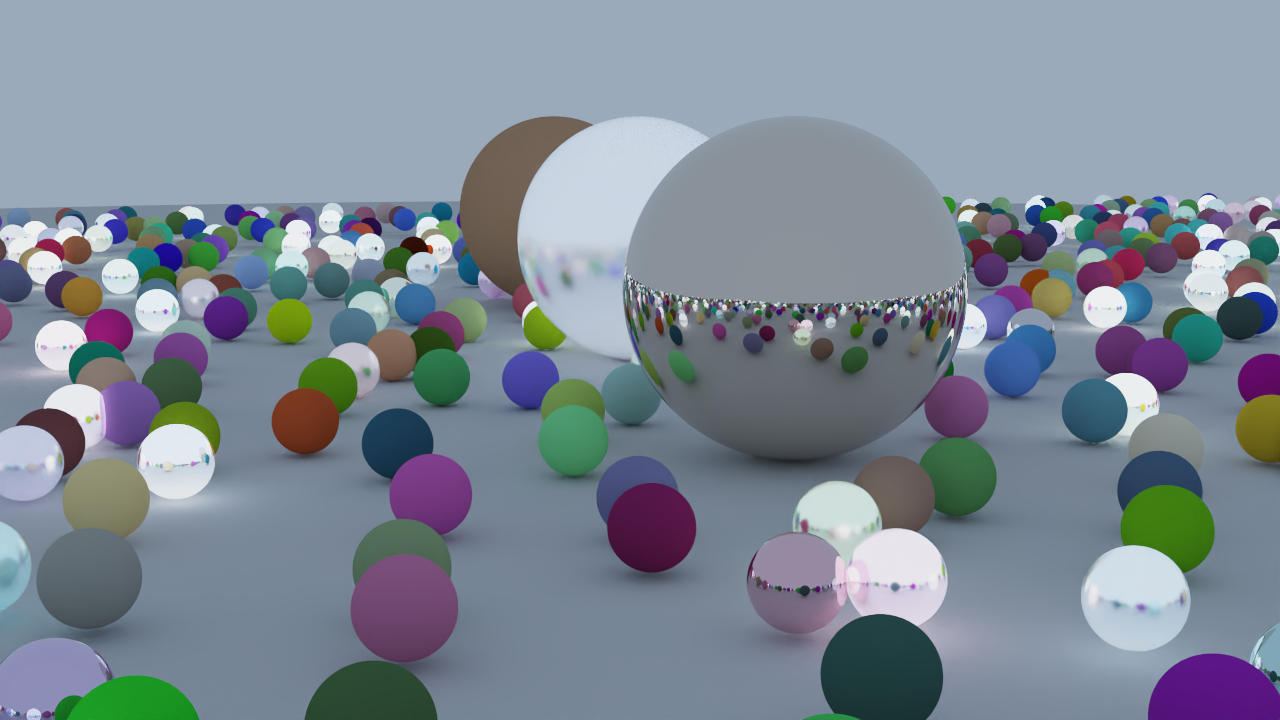
\includegraphics[width=0.78\textwidth]{bvh-scene.png}
  \caption{Cena de demonstração da BVH (\texttt{VI-RT bvh}): ${\approx}1300$ esferas, 64 spp + OIDN. Render: \SI{38}{s} com BVH; ${\approx}11$ min com a grelha.}
  \label{fig:bvhscene}
\end{figure}

\begin{figure}[H]
  \centering
  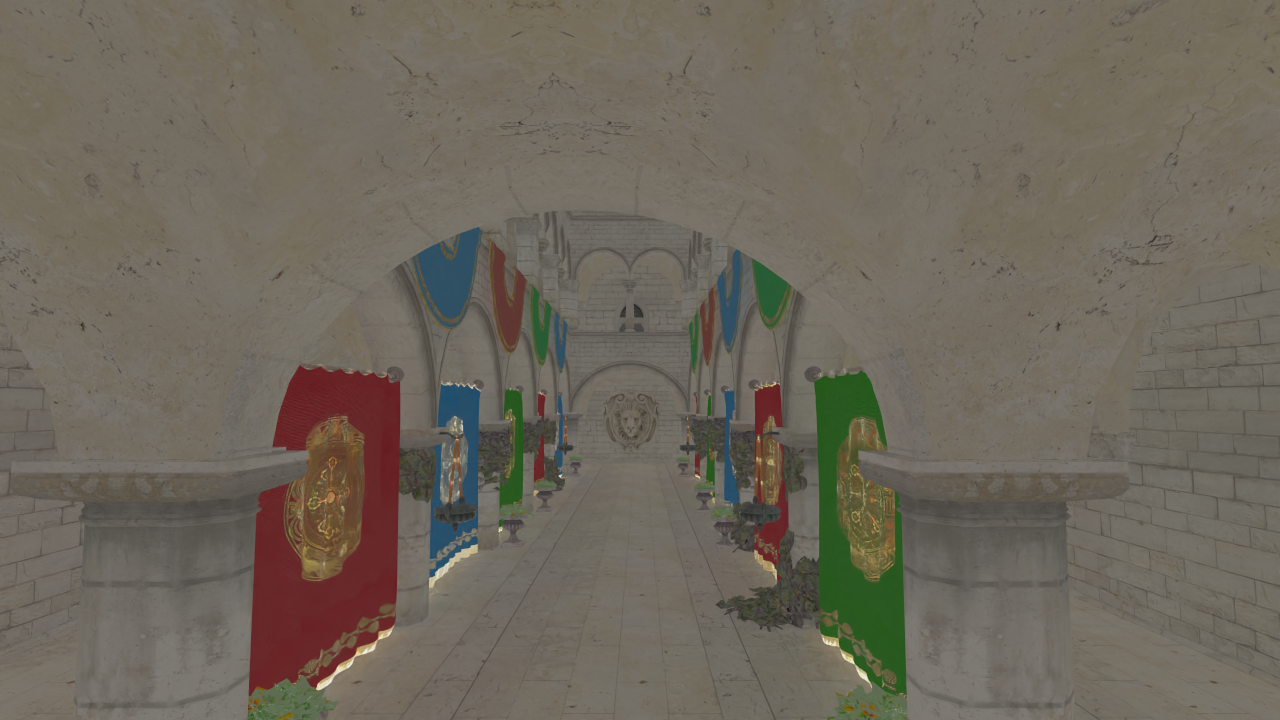
\includegraphics[width=0.78\textwidth]{sponza-interior.png}
  \caption{Sponza (262\,mil triângulos), vista interior, 24 spp + OIDN --- geometria real onde a BVH de triângulos é decisiva.}
  \label{fig:sponza}
\end{figure}


% ============================================================================
% ========================= TEMA 5 — DEPTH OF FIELD ==========================
% ====================== [SECÇÃO DE: NOME DA COLEGA] =========================
% ============================================================================

\section{Tema 5 --- Depth of Field}
\label{sec:dof}

% TODO [colega]: escreve aqui a tua parte. Estrutura sugerida:

\subsection{Fundamento}

% TODO [colega]: câmara pinhole vs lente com abertura finita, círculo de confusão,
% modelo de lente fina (referência: Ray Tracing in One Weekend \cite{rtiow}).

[A preencher.]

\subsection{Implementação}

% TODO [colega]: parâmetros defocus_angle e focus_dist na Camera, viewport no
% plano focal, amostragem do disco da lente em GenerateRay.

[A preencher.]

\subsection{Resultados}

% TODO [colega]: 2-3 renders variando defocus_angle (ex.: 0°, 0,6°, 2°) com o
% mesmo focus_dist; sugestão de cena: VI-RT bvh ou o Sponza (estandartes em
% profundidade). Nota: o DoF multiplica os samples necessários — podes referir
% que a BVH (secção \ref{sec:bvh}) torna isso praticável.

[A preencher.]

% ============================================================================

\section{Conclusão}

% TODO [grupo]: completar quando as três secções estiverem fechadas.
% Esqueleto sugerido:

Os três temas formam um \emph{pipeline} coerente de ``fotografia virtual'': o \emph{motion blur} e o \emph{depth of field} acrescentam realismo físico à câmara, ambos à custa de mais amostragem estocástica; a BVH reduz o custo dessa amostragem em mais de duas ordens de grandeza (${\approx}245\times$ na cena mais pesada), mantendo resultados bit a bit idênticos. [Completar com as conclusões dos temas 5 e 6.]

\paragraph{Divisão do trabalho.} Motion Blur --- [NOME]; BVH --- Gonçalo Barroso; Depth of Field --- [NOME].

\begin{thebibliography}{9}

\bibitem{pbrt}
M.~Pharr, W.~Jakob, G.~Humphreys,
\emph{Physically Based Rendering: From Theory to Implementation},
3.ª~ed., Morgan Kaufmann, 2016 --- cap.~4 (BVH).

\bibitem{rtiow}
P.~Shirley, T.~Black, S.~Hollasch,
\emph{Ray Tracing in One Weekend} --- Defocus Blur.
\url{https://raytracing.github.io/books/RayTracingInOneWeekend.html}

\bibitem{rtnw}
P.~Shirley, T.~Black, S.~Hollasch,
\emph{Ray Tracing: The Next Week} --- Motion Blur; Bounding Volume Hierarchies.
\url{https://raytracing.github.io/books/RayTracingTheNextWeek.html}

\bibitem{oidn}
Intel Open Image Denoise.
\url{https://www.openimagedenoise.org}

\end{thebibliography}

\end{document}
